\pagestyle{kalinka}
\label{kalinka}

\begin{textblock*}{5.625in}(0pt,0pt)%
\vspace*{-3.49cm}
\hspace*{-2.76cm}\includegraphics*[width=175.2mm]{./propagandas/KALINKA.pdf}
\end{textblock*}

\pagebreak %A CIDADE ENE

\begin{center}
\hspace*{-3.6cm}\raisebox{5cm}{\rotatebox[origin=t]{90}{\huge\Formular{\textbf{Lançamento}}}}
\hspace*{3.1cm}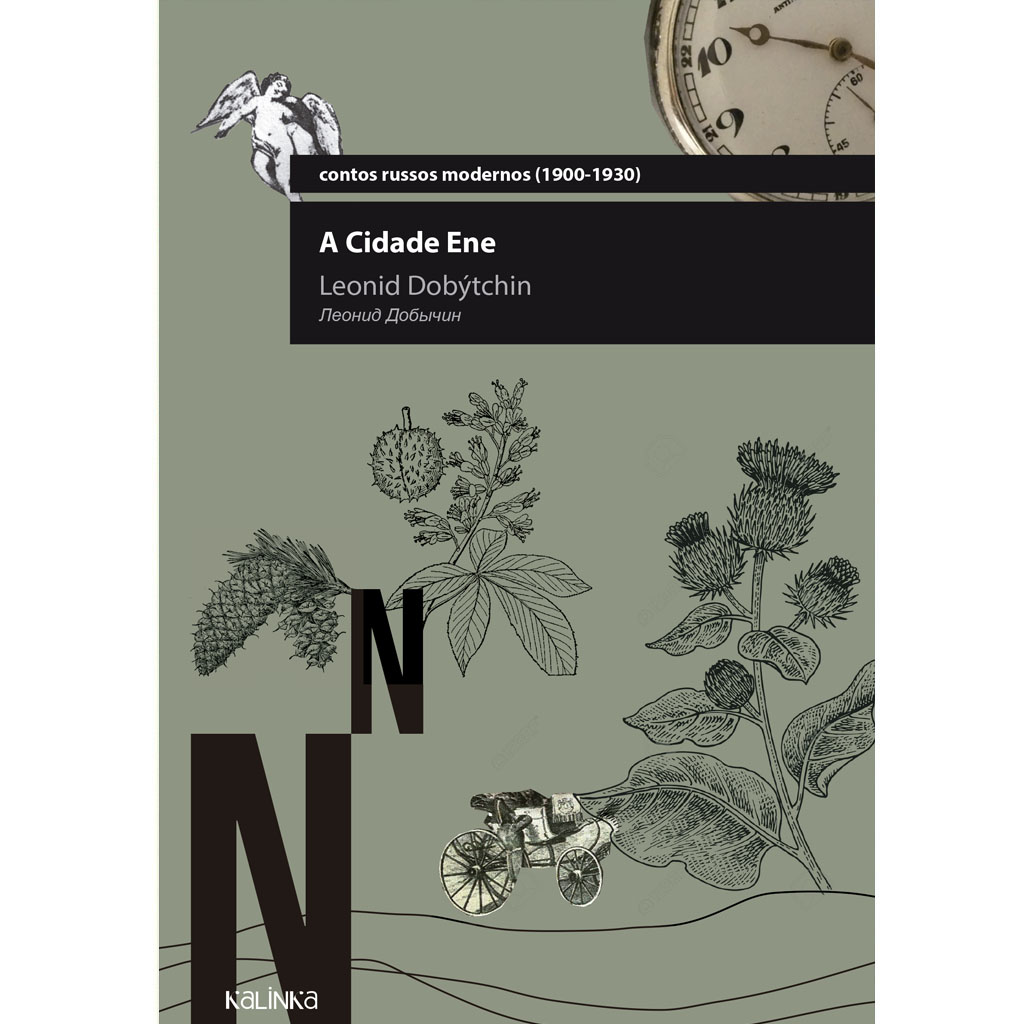
\includegraphics[width=74mm]{./grid/cidaden.jpg}
\end{center}

\hspace*{-7cm}\hrulefill\hspace*{-7cm}

\medskip

\noindent{}\hlc[lightyellow]{A Cidade Ene'' é uma narrativa do ponto de vista de uma criança do começo do século XX. Desvelam"-se reminiscências de uma Rússia pré"-revolucionária e sua burguesia decadente e provinciana.} Na fictícia cidade Ene --- em homenagem à cidade de {\slsc{Almas mortas}} de Gógol --- são percebidas fortes características de Daugavpils, onde o autor Leonid Dobýtchin viveu boa parte da vida. Embora seja também um lugar simbólico, um todo"-lugar, representando o conjunto dos ambientes urbanos russos: ao buscar continuidades, questiona"-se a real profundidade produzida pela Revolução  no homem e na sociedade.

Com uma das histórias mais trágicas da história literária russa, já repleta de infortúnios, o autor não teve sua própria mesa para escrever até os 40 anos, quando recebeu da União dos Escritores Soviéticos um quarto num apartamento comunal em São Petersburgo, dois anos antes de falecer em presumido suicídio. Perseguido pela máquina de censura stalinista, foi taxado como “formalista”. Ele se defendeu das acusações e desapareceu no dia seguinte, nunca mais ninguém o viu.

\vfill

\hspace*{-.4cm}\begin{minipage}[c]{.5\linewidth}
\small{
{\Formular{\textbf{
\hspace*{-.1cm}Editora: Kalinka\\
Título: A Cidade Ene\\
Autor: Leonid Dobýtchin\\ 
ISBN: 978-65-8686-200-3\\
Páginas: 142\\
Formato: 14x21cm\\
Preço: R\$ 42,90\\
Disponibilidade: 24/07/2020
}}}}
\end{minipage}


\pagebreak

\vspace*{1.5cm}

\noindent{}{\nohyphens{\LARGE{Livro fatídico}}}

\bigskip

\hfill{}\scalebox{.8}{VALÉRI SÁJIN}

\bigskip
\bigskip
\bigskip

\begin{multicols}{2}
Leonid Dobýtchin publica seus primeiros contos aos trinta anos, quando, no fim do verão de 1924, remeteu duas narrativas curtas ao acaso para a revista leningradense {\slsc{O contemporâneo
russo}} ({\slsc{Rússkii sovremiénnik}}), que são quase imediatamente publicados.
Alí caiu em boas mãos. Foi apadrinhado por escritores não
estranhos a inovações literárias (por vezes oficialmente): Kornei
Tchukóvski e seu filho Nikolai, Mikhail Slonímski, Veniamin Kaviérin e
outros prosadores de Leningrado. Eles aceitaram e incentivaram o estilo
distanciado de Dobýtchin, contribuíram para a publicação de seus contos
e para a apresentação do escritor em dezembro de 1929 na União dos
Escritores de Toda a Rússia.

Mas vez ou outra censuravam a brevidade,
assim a julgavam, de suas obras e insistiam para que ele escrevesse um
romance (por algum motivo justamente um romance). Dobýtchin tentava
corresponder aos desejos de seus protetores. De 1926 a 1932 ele de
tempos em tempos lhes informava que estava ``terrivelmente empenhado''
em escrever um romance, mas logo reconhecia com tristeza que não passava
das ``700 palavras''. Para Dobýtchin o problema consistia na visível
limitação do espaço físico de sua existência (a provinciana Briansk com sua população de oitenta e poucos mil habitantes) e
--- como se depreende de seus contos fartos de realidades concretas ---
em sua aversão absoluta à ``invenção''. Com esse paradigma como seria
possível encontrar material para a criação de uma obra volumosa e
orgânica?

O escritor o achou em seu passado: nas recordações de sua própria
infância.

Dobýtchin nasceu em 5 (17 no calendário gregoriano) de junho de 1894. Desde os dois anos passou a
viver com os pais na Rússia ocidental, na cidade de Dvinsk, parte da
província de Vítebsk (em dezembro de 1917 os bolcheviques transferiram a
cidade para a Letônia soviética e em 1920 a nomearam Daugavpils). Aos
oito anos Leonid perdeu o pai, que trabalhava como médico. Sua mãe, que
havia concluído o Instituto de Obstetrícia em Petersburgo, cuidava da
família, mas, depois da morte do marido, viu"-se obrigada a trabalhar
como parteira. Em 1911, ao concluir a {\slsc{escola real}} de Dvinsk,
Leonid ingressou no Departamento de Economia do Instituto Politécnico de
Petersburgo. Sua especialidade tornou"-se a estatística. Na primavera de
1918, algum tempo depois de sua mãe ter se mudado de Dvinsk para
Briansk, Dobýtchin aqui se estabeleceu e praticamente até o final de sua
vida --- com
intervalos --- trabalhou em diversos institutos de estatística
da cidade.

\bigskip

{\small\fakereceipt{
“Por trás do número enorme de personagens, topônimos,
fatos históricos e outros detalhes da história narrada em
\emph{A Cidade Ene}, está o relato de uma busca comovente e incansável de
uma criança por um amigo”
}}

\bigskip

Em maio de 1933 Dobýtchin finalmente enviou a Leningrado alguns dos
primeiros capítulos do ``romance''. Eles só puderam ser publicados
exatamente um ano depois, no quinto número (maio) da revista {\slsc{Terra
virgem vermelha}} ({\slsc{Krásnaia nov}}). Os treze capítulos da obra nova
--- e insolitamente grande para os leitores familiarizados com a prosa
de Dobýtchin --- receberam um título ``de gênero'' incomum: ``O início
de um romance''. Um ano e meio depois, em novembro/dezembro de 1935, com
o acréscimo de vinte e um novos capítulos ao anterior ``O início de um
romance'', o livro de Dobýtchin saiu já com o título {\slsc{A Cidade Ene}}
(importante: sem indicação do gênero da obra). Era uma narrativa
autobiográfica sobre sua infância em Dvinsk.

Os trinta e quatro capítulos de {\slsc{A Cidade Ene}} reproduzem em
detalhes exatamente dez anos da vida do autor"-narrador: dos seis aos
dezesseis anos de idade. A série de acontecimentos mencionados permite
inferir a extensão temporal do texto, de 1901 a 1911: no capítulo onze
se descreve uma exposição agrícola (ela ocorrera em 1903 em Dvinsk);
depois se mencionam o início da guerra com o Japão (1904) e sua
conclusão (agosto de 1905); a revolução 
na Turquia (1908); em 
seguida o
centenário do nascimento de Gógol (março de 1909); a morte de Lev
Tolstói (7 de novembro de 1910); o voo do aviador Serguei Útotchkin, que
sobrevoou Dvinsk pela primeira vez em 1º de junho de 1911\ldots{} No
intervalo entre os eventos enumerados, é mencionada uma quantidade
enorme de acontecimentos locais de Dvinsk, da Rússia e do exterior que
estão impregnados na trama historicamente precisa da {\slsc{Cidade Ene}}
(com raros deslocamentos cronológicos).

Uma questão pode parecer estranha: em que {\slsc{A Cidade Ene}} se
diferencia das obras conhecidas anteriores de Dobýtchin? A resposta deve
ser simples: no volume e na ausência do farto contexto soviético,
impossível em uma narrativa com episódios do comecinho do século \scalebox{.8}{XX}. Com
efeito. O paradoxo de {\slsc{A Cidade Ene}} no entanto consiste no fato de
que a nova obra de Dobýtchin reproduz em minúcias os procedimentos
principais de suas miniaturas precedentes. Se antes eles estavam
diluídos em uma dezena de textos, agora aparecem de forma concentrada.

Da mesma forma que Dobýtchin em seus contos assinalou escrupulosamente
os topônimos no espaço em que se desenrolava a ação, em {\slsc{A Cidade
Ene}} o leitor praticamente em cada capítulo é informado exatamente onde
e em que momento a ação se desenrola ou quais objetos se encontram no
campo de visão do menino"-narrador: o castelo"-prisão, a fortaleza
militar, o teatro e o cinema, a estação e a rua ``dos prazeres'' nos
arredores da estação, o viaduto sobre a estrada de ferro para a passagem
de uma parte da cidade à outra\ldots{} São elementos reais de Dvinsk, e
nenhum deles, ao que parece, escapou à narrativa de Dobýtchin.

Com eles se conjugam motivos religiosos, característicos dos eventos de
praticamente todos os contos de Dobýtchin. Em {\slsc{A Cidade Ene}}, temos
as menções obrigatórias aos templos católicos ({\slsc{kostiol}}), às
catedrais ortodoxas, às igrejas luteranas e aos templos dos {\slsc{velhos
crentes}} (Dvinsk era uma cidade multinacional e multiconfessional), e,
quando a ação por vezes se desloca da cidade natal do menino para outro
espaço, inevitavelmente se indicam os templos locais. Além disso, com
frequência, de capítulo em capítulo (em vinte e nove dos trinta e
quatro!), são descritos ritos e festejos religiosos, e não apenas uma
vez é citado o Novo Testamento (por sinal, Dobýtchin o citava largamente
em suas correspondências)\ldots{} Pode"-se dizer que toda a vida do narrador,
de uma ou de outra maneira, está mergulhada nessa atmosfera religiosa.

Como é evidente, nos enredos dos contos de Dobýtchin sistematicamente
surge a morte de uma ou de outra personagem, e nos enterros (ou nos
feriados) tocam orquestras. Em {\slsc{A Cidade Ene}} o leitor desde o
começo ``escuta'' uma orquestra militar e depois, de capítulo em
capítulo, orquestras acompanham a narrativa.~O mesmo ocorre quanto aos
funerais e cemitérios: a partir do segundo capítulo, mortes, funerais e
cemitérios são circunstâncias invariáveis da vida do menino.

O caráter ``literocêntrico'' um pouco velado de seus contos
(menção a Nikolai Gógol em ``Sávkina'', a Oscar Wilde e Upton Sinclair
em ``Dorian Gray'', a Serguei Essiénin em ``O retrato'', e aparições
frequentes de bibliotecas ou ``bibliotecárias'' em vários contos) é
solidamente acentuado em {\slsc{A Cidade Ene}}. Isso se expressa por meio
de referências contínuas a nomes e a obras de escritores russos e
estrangeiros (praticamente vinte, contando por alto) feitas pelo
narrador"-bibliófilo, que ``não tinha assunto'' com alguém de sua idade
que não lesse. E, o principal, o motivo que perpassa o livro é dado já
no título. {\slsc{A Cidade Ene}} é o espaço gogoliano de {\slsc{Almas
mortas}}. A personagem principal de Dobýtchin faz sistematicamente
ligações com o poema de Gógol e volta e meia se identifica com o herói
Tchítchikov, desejando mudar"-se para a formidável cidade Ene ({\slsc{N}}
em Gógol). O que o atrai? O exemplo da amizade terna de Tchítchikov e
Manílov e o desejo de tornar"-se amigo dos filhos de Manílov.

Pode"-se dizer assim que, por trás do número enorme de personagens, topônimos,
fatos históricos e outros detalhes da história narrada por Dobýtchin em
{\slsc{A Cidade Ene}}, está o relato de uma busca comovente e incansável de
uma criança por um amigo.

\bigskip

\textcolor{gray}{\footnotesize\slsc{Adaptado do prefácio do livro “A Cidade Ene”. Tradução de Moissei Mountian.}}
\end{multicols}

\pagebreak
\pagestyle{kalinkacat}

\begin{multicols}{2}
\begin{enumerate}
\raggedright\nohyphens{
\item O compromisso, {\Formular{\textbf{Serguei Dovlátov}}}
\item Aulas de literatura russa, {\Formular{\textbf{Aurora Fornoni Bernardini}}}
\item O Elefante, {\Formular{\textbf{Aleksandr Kuprin}}}
\item A Velha, {\Formular{\textbf{Daniil Kharms}}}
\item Bobok E Meia Carta De Um Sujeito, {\Formular{\textbf{Fiódor Dostoiévski}}}
\item Parque cultural, {\Formular{\textbf{Serguei Dovlátov}}}
\item O diabo mesquinho, {\Formular{\textbf{Fiódor Sologub}}}
\item Tarakã, o bigodudo, {\Formular{\textbf{Kornei Tchukóvski}}}
\item Salmo, {\Formular{\textbf{Friedrich Gorenstein}}}
\item O Oficio, {\Formular{\textbf{Serguei Dovlátov}}}
\item Luminescência, {\Formular{\textbf{Viatchesláv Kupriyánov}}}
\item Poesia russa, {\Formular{\textbf{Vários}}}
\item Encontros com Liz e outras histórias, {\Formular{\textbf{Leonid Dobýtchin}}}
\item Os sonhos teus vão acabar contigo, {\Formular{\textbf{Daniil Kharms}}}
}
\end{enumerate}
\end{multicols}

\pagebreak




%\hspace{.5cm}
%
%\begin{center}
%\hspace*{-1cm}\raisebox{5.5cm}{\rotatebox[origin=t]{90}{\Formular{\textbf{Lançamento}}}}
%\hspace{1cm}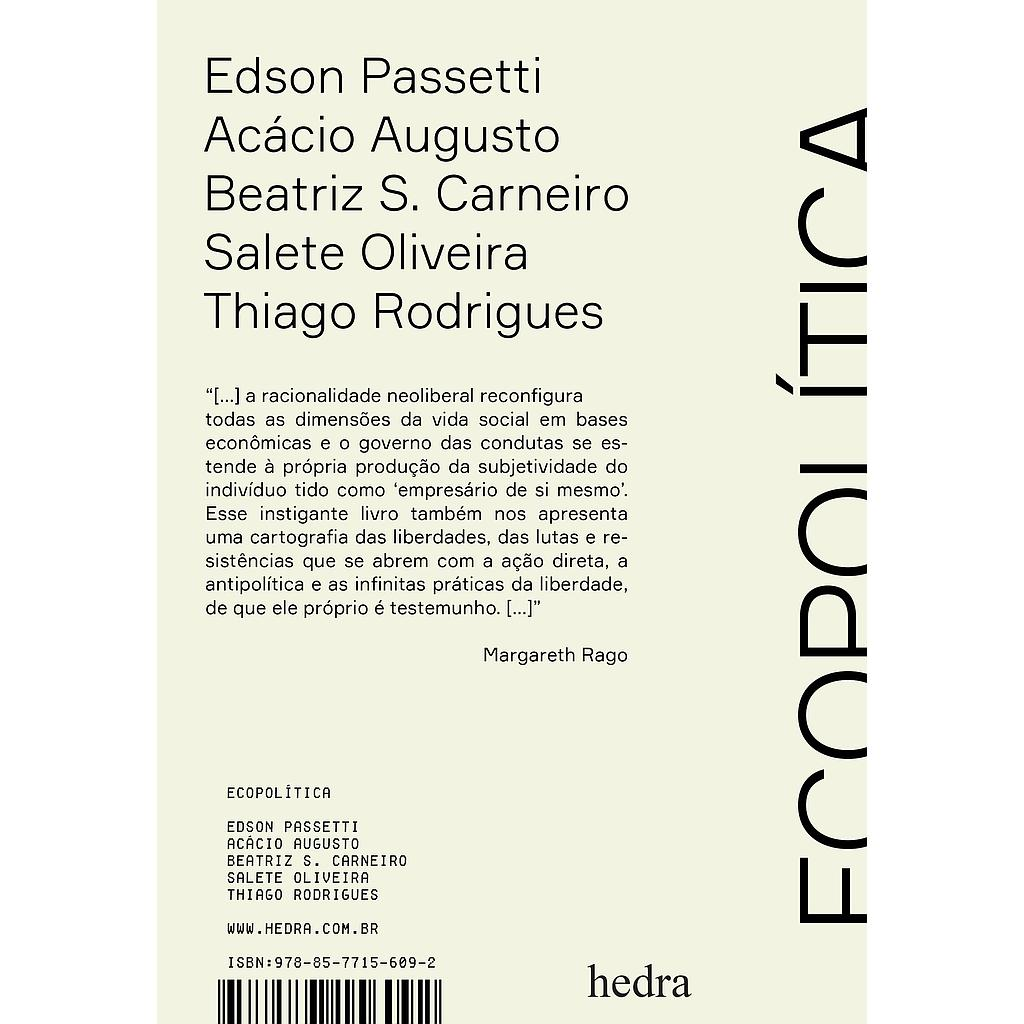
\includegraphics[width=70mm]{eco.jpeg}
%\end{center}
%
%\hspace*{-2cm}\_\_\_\_\_\_\_\_\_\_\_\_\_\_\_\_\_\_\_\_\_\_\_\_\_\_\_\_\_\_\_\_\_\_\_\_\_\_\%_\_\_\_\_\_\_\_\_\_\_\_\_\_\_\_\_\_\_\_\_\_\_\_\_\_\_\_\_\_\_\_\_\_\_\_
%
%\medskip
%
%\noindent{}Lorem ipsum dolor sit amet, consectetur adipiscing elit.
%Donec sodales tortor a purus accumsan, ut ultricies purus
%maximus. Aliquam bibendum consequat mi, sed commo-
%do velit pellentesque id. Vivamus ultricies ligula in semper
%sagittis. Donec mollis odio in lectus tristique, sed convallis
%est interdum. Cras eget sem condimentum, pretium purus
%eu, auctor.
%
%\hspace{.5cm}
%
%\hspace*{-.4cm}\begin{minipage}[c]{0.45\linewidth}
%\small{
%{\Formular{\textbf{
%\hspace*{-.1cm}Título: Ecopolítica\\
%Autor: Edson Passetti\\ 
%Editora: Hedra\\
%Páginas: 476\\
%Formato: 23x16cm\\
%Preço: R\$ 79,90\\
%}}}}
%\end{minipage}
%\begin{minipage}[c]{0.50\linewidth}
%\small{Lorem ipsum dolor sit amet, consectetur adipiscing elit. Donec sodales tortor a purus accumsan, ut ultricies. Lorem ipsum dolor sit amet, %consectetur adipiscing elit. Lorem ipsum dolor sit amet. Lorem ipsum dolor sit amet.} 
%\end{minipage}
%
%\pagebreak
%
%\hspace{.5cm}
%
%\begin{center}
%\hspace*{-.5cm}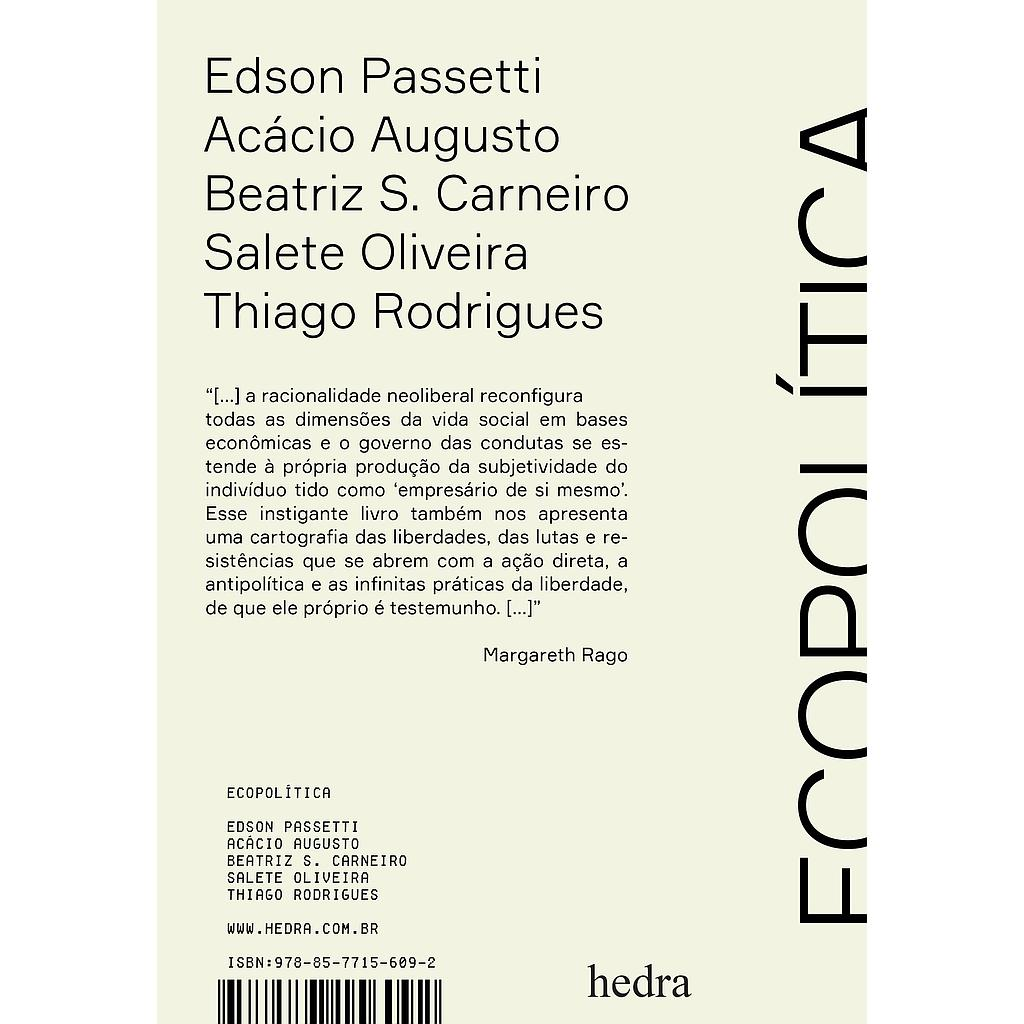
\includegraphics[width=70mm]{eco.jpeg}
%%\hspace*{6cm}\raisebox{2cm}{\rotatebox[origin=t]{90}{\Formular{\textbf{Lançamento}}}}
%\end{center}
%
%\hspace*{-2cm}\_\_\_\_\_\_\_\_\_\_\_\_\_\_\_\_\_\_\_\_\_\_\_\_\_\_\_\_\_\_\_\_\_\_\_\_\_\_\%_\_\_\_\_\_\_\_\_\_\_\_\_\_\_\_\_\_\_\_\_\_\_\_\_\_\_\_\_\_\_\_\_\_\_\_
%
%\medskip
%
%\noindent{}Lorem ipsum dolor sit amet, consectetur adipiscing elit.
%Donec sodales tortor a purus accumsan, ut ultricies purus
%maximus. Aliquam bibendum consequat mi, sed commo-
%do velit pellentesque id. Vivamus ultricies ligula in semper
%sagittis. Donec mollis odio in lectus tristique, sed convallis
%est interdum. Cras eget sem condimentum, pretium purus
%eu, auctor.
%
%\hspace{.5cm}
%
%\hspace*{-.4cm}\begin{minipage}[c]{0.45\linewidth}
%\small{
%{\Formular{\textbf{
%\hspace*{-.1cm}Título: Ecopolítica\\
%Autor: Edson Passetti\\ 
%Editora: Hedra\\
%Páginas: 476\\
%Formato: 23x16cm\\
%Preço: R\$ 79,90\\
%}}}}
%\end{minipage}
%\begin{minipage}[c]{0.50\linewidth}
%\small{Lorem ipsum dolor sit amet, consectetur adipiscing elit. Donec sodales tortor a purus accumsan, ut ultricies. Lorem ipsum dolor sit amet, %consectetur adipiscing elit. Lorem ipsum dolor sit amet. Lorem ipsum dolor sit amet.} 
%\end{minipage}
%
%\pagebreak